% !TeX root = ../main.tex

\xchapter{智能光电处理算法与系统设计研究基础}{Research Foundation of Intelligent Electro-Optical  Algorithms and System Design}
本章主要介绍智能光电系统的基本组成以及其中涉及的到核心功能,目标检测和目标跟踪的相关算法研究基础。

\xsection{智能光电系统基本组成}{Fundamental Architecture of Intelligent Electro-Optical Systems}
智能光电系统,作为无人机实现环境感知与智能决策的核心,是一个深度融合了光学、机械、电子、计算机与人工智能的复杂综合性系统。其基本工作原理是建立在光电转换与信息处理的基础之上,系统通过各类光电传感器,捕获目标反射或辐射的电磁波信号,经由一系列软硬件模块的处理,完成光信号到电信号的初级转换。现代智能光电系统的关键差异在于其信息处理架构的改变:它将传统上由地面站或后端服务器承担的高级处理功能(如图像增强、特征提取、目标识别与跟踪)前移至机载端侧。这一转变的核心在于系统内部集成了高性能的嵌入式计算平台(如Nvidia Jetson系列,华为Atlas系列,瑞芯微RK系列),能够在数据产生的源头对原始图像进行实时、智能化的处理与分析,直接形成可供决策的结构化信息。这种一体化设计,不仅极大降低了对数据链带宽的依赖,减少了信息传输的延迟,更使无人机平台获得了在复杂、动态环境中进行即时态势理解和自主响应的能力,从而真正实现了从“被动成像设备”到“主动感知节点”的智能化跃迁。


智能光电系统的硬件架构是实现其物理功能的基础,通常遵循模块化、集成化设计原则,以适应无人机平台对载荷尺寸、重量和功耗的严苛限制。其核心硬件模块主要包括光学传感单元、惯性稳定平台以及信息处理单元。

光学传感单元负责从环境中捕获原始光学信息。为突破单一波段感知的局限,满足全天候、全时段及复杂场景下的探测需求,现代光电系统的演进方向已从早期的单一传感器,发展为多光谱、多传感器深度融合的架构。可见光高清成像与长波热红外成像系统已逐渐成为现代机载光电系统的标配,可见光成像系统通常基于高分辨率的CCD或CMOS图像传感器构建,配备电动连续变焦镜头,以实现从广域搜索到细节识别的无缝切换。其作用是在昼间良好光照条件下提供富含纹理和色彩信息的高清图像。红外热成像系统是系统实现夜间和恶劣气象条件下工作的关键,它们通过探测目标与背景的热辐射差异来生成热图像。在此基础上,为进一步提升系统在复杂环境下的感知能力,现代光电系统还逐步集成中波红外、短波红外、微光、多光谱成像仪激光测距仪等特种传感器。中波红外传感器对高温目标(如发动机喷口、导弹尾焰)极为敏感,是实现早期预警与精准识别的关键,短波红外传感器具有穿透薄雾、烟尘和水汽的能力,提升系统在恶劣天气下的感知能力,微光传感器能在极低照度下将微弱光子信号大幅增益,生成可供人眼判读的夜景图像。多光谱成像仪能在多个狭窄、连续的波段内同时对目标成像,从而提升对伪装目标、特定物质的识别与分类能力,激光测距仪通过测量激光脉冲的往返时间精确计算目标距离,为定位提供关键参数。
机载光电系统主要用于对地面目标进行识别跟踪、激光测距和照射等,主要指标包括以下部分或全部:红外作用距离、红外探测视场、红外探测波长、可见光作用距离、可见光探测视场、可见光探测波长、稳定精度、跟踪精度、随动精度、瞄准线指示精度、搜索范围、搜索角速度、搜索角加速度、跟踪速度、跟踪加速度、视场切换时间、激光工作波长、激光测距范围、激光照射距离、激光照射频率、激光照射精度、光轴平行度、工作准备时间、供电电源、系统重量和外形尺寸等。
其中与光学传感单元相关的最重要的系统指标是可见光与红外作用距离,下面将具体分析这两个指标

\subsubsection{红外作用距离}
人眼通过显示器看到红外成像系统获得的目标图像的基本条件包括:1. 目标具有一定空间频率。2. 目标与背景的温差经过大气衰减,到达红外系统探测器上时仍大于或等于系统对该频率的最小可分辨温差(MRTD),即
\begin{equation}
\left\{\begin{array}{l}\Delta T=\Delta T_{\mathrm{e}} \cdot \tau_{\mathrm{a}} \geqslant \operatorname{MRTD}(f) \\ \frac{H}{2 n_{\mathrm{e}} \cdot R} \geqslant \theta\end{array}\right.
\end{equation}

其中,$\Delta T$为经过大气衰减后,目标与背景的温差,$\Delta T_{\mathrm{e}}$为目标与背景的实际温差,$\tau_{\mathrm{a}}$为R距离上的大气平均透过率,MRTD(f)为系统对空间频率f的最小可分辨温差,H为目标尺寸,$n_{\mathrm{e}}$为不同观察等级要求时的目标等效线对数,R为目标与系统的距离,$\theta$为瞬时视场。

对于目标的发现距离和识别距离,目前光电系统都是根据JOHNSON法则,即发现目标和识别目标50\%概率所需线对数$n_{\mathrm{e}}$,

\begin{table}[H]
% \setlength{\abovecaptionskip}{-6pt}
\caption{JOHNSON法则规定的发现和识别判据}
\centering
\begin{center}
\begin{tabularx}{0.8\textwidth}{*{2}{Y}}
\toprule
鉴别等级 & 50\%概率所需线对数 \\ \midrule
发现 & 1.0 $\pm$ 0.25 \\
识别 & 4.0 $\pm$ 0.8 \\
\bottomrule
\end{tabularx}
\label{JOHNSON}
\end{center}
\end{table}

红外系统的瞬时视场由探测器面元数量和总视场决定,表达式为
\begin{equation}
\theta=\frac{\alpha}{n}
\end{equation}

其中,$\alpha$为系统偏航或俯仰方向的总视场,n为探测器偏航或俯仰方向的面元数量。

由上可知,红外系统在设计中既要考虑能量方面的要求,又要考虑空间分辨率的要求,MRTD是一个综合考核的指标,可以综合描述系统的空间分辨率和温度灵敏度特性,与目标的空间频率、系统传递函数和等效噪声温差等相关。一般情况下,对于近距离探测目标,红外系统空间分辨率是主要矛盾,对于远距离探测目标,温度灵敏度即能量因素是主要矛盾。

\subsubsection{可见光作用距离}
可见光探测利用的是目标对阳光的反射光,与红外探测相似,获得可观察的目标图像的基本条件是:1. 具有一定空间频率的目标,2. 经过大气衰减后到达CCD的照度满足最低照度要求,目标与背景的对比度经大气衰减后满足成像要求。即空间分辨能力和能量分辨能力,具体理论计算公式为

\begin{equation}
    \left\{\begin{array}{l}
E=\frac{1}{4} E_0 \rho_{\mathrm{t}} \tau_{\mathrm{a}} \tau_0\left(\frac{D}{f}\right)^2 \geqslant E_{\mathrm{M}} \\
C=C_0 \cdot \tau_{\mathrm{a}} \cdot \tau_0 \geqslant C_{\mathrm{M}} \\
\frac{H}{2 n_{\mathrm{e}} \cdot R} \geqslant \theta
\end{array}\right.
\end{equation}

其中,E为到达CCD像面的照度,$E_0$为环境照度,$\rho_{\mathrm{t}}$为目标反射率,$\tau_{\mathrm{a}}$为大气透过率,$\tau_0$为系统光学透过率,$\frac{D}{f}$为可见光系统相对孔径,$E_{\mathrm{M}}$为CCD工作允许的最低照度,C为经过大气传输后目标与背景的对比度,$C_0$为目标与背景的对比度,$C_{\mathrm{M}}$为人眼能够分辨的最低对比度,H为目标尺寸,$n_{\mathrm{e}}$为不同观察等级要求时的目标等效线对数,R为目标与系统的距离,$\theta$为瞬时视场。 


惯性稳定平台是机载光电系统硬件架构中实现高精度指向与稳定成像的核心模块,其核心功能在于隔离无人机飞行中的高频振动、姿态变化等运动干扰,为光学传感器提供一个相对稳定的基准,从而确保获取清晰、稳定的图像与视频数据。为实现这一目标,平台在机械上通常采用精密的框架式结构,例如常见的两轴(方位、俯仰)四环架设计:内万向架直接承载并稳定光电传感器,尽可能隔离载体振动,外万向架则将内环与外部环境扰动进一步隔离。该系统主要由框架结构、敏感测量元件、伺服驱动机构及控制单元组成。敏感元件(如陀螺仪)实时测量载体或框架自身的角运动,这些运动信息被送至控制单元(如基于单片机的数字控制器)。控制单元计算补偿指令,并驱动安装在框架轴上的力矩电机产生反向力矩,从而主动抵消扰动,使光电传感器的视轴在惯性空间中保持稳定锁定或实现平滑跟踪。随着技术发展,为在性能与体积重量间取得更好平衡,出现了“半捷联稳定”等先进形式,其利用载机惯性导航系统的信息辅助稳定,减少了平台上的陀螺数量,有助于实现系统的小型化和轻量化。惯性稳定平台的设计与性能,直接决定了整个机载光电系统在动态环境下成像的清晰度、目标跟踪的准确性。

智能机载光电系统的信息处理单元已超越简单的数据采集与转发,成为一个集采集,处理,智能分析于一体的综合模块。它不仅负责采集来自可见光、红外、激光等多种传感器的海量数据并进行去噪、增强、稳像等预处理,还需在尺寸、重量和功耗严格受限的机载环境下,完成目标检测、跟踪及多传感器融合等复杂的计算任务。现代信息处理单元普遍采用异构计算架构,主流设计通常集成通用CPU用于复杂逻辑与控制、高性能GPU用于并行图像处理与AI推理、专用神经网络处理器NPU用于高效执行深度学习算子。在工程实现上,常使用FPGA作为高速数据采集、预处理和逻辑控制的协处理器,与AI主控芯片构成异构系统,以实现性能与效率的最佳平衡。为适配各类传感器,处理单元还提供丰富的工业级接口,如多路MIPI CSI(相机串行接口)、GMSL(千兆多媒体串行链路)用于摄像头接入,以及CAN总线、ETH、RS-232/422/485等用于与其他设备通信。在具体产品形态上,信息处理单元常以核心计算模组(System on Module, SOM)或整机系统的形式存在。下面列举几种面向高性能边缘计算场景的代表性模组:

\begin{table}[H]
% \setlength{\abovecaptionskip}{-6pt}
\caption{边缘计算模组}
\centering
\begin{center}
% \begin{tabularx}{\textwidth}{*{3}{Y}}
\begin{tabularx}{\textwidth}{p{2.5cm}XX}
\toprule
模组名称 & 核心架构与算力 & 关键特性 \\ \midrule
Nvidia Jetson & CPU + CUDA核心 + Tensor核心,算力覆盖数TOPS至数百TOPS & 拥有最成熟的CUDA开发生态,提供从开发、部署、调试的全栈工具,便于复杂神经网络的部署。平台丰富(如Nano,Xavier,NX,Orin,Thor) \\
华为Ascend & 昇腾CPU + 达芬奇架构NPU,Atlas 200I A2模块提供8-20 TOPS INT8算力 & 高集成度与能效比,单模块集成CPU、AI计算、编解码等功能。全国产化,适用于有自主可控要求的项目 \\
瑞芯微RK & ARM架构CPU + 自研NPU,提供1-6 TOPS INT8算力,内置高性能ISP & 强大的多媒体处理与接口能力,支持多路摄像头输入和8K编解码。高性价比与低功耗,内置ISP简化了成像系统设计。支持多种操作系统和开发框架,适用于轻量级AI应用 \\
寒武纪MLU & 基于寒武纪MLUv02架构的专用AI推理模组,提供16 TOPS INT8峰值算力 & 专为边缘AI设计,支持主流深度学习框架,低功耗、紧凑型设计,是AI核心硬件国产化替代的选项之一 \\
\bottomrule
\end{tabularx}
\label{edge-device}
\end{center}
\end{table}

\xsection{机载光电系统目标检测算法研究基础}{Overview of Object Detection Algorithms}

目标识别是指在图像或视频序列中检测并定位特定类别的目标物体。这一过程超越了单纯感知图像内容,上升至对场景的理解层次。对于机载光电系统而言,目标识别是实现智能感知、态势理解与自主决策的基石,其性能直接决定了无人机能否在复杂的低空环境中,从海量图像数据中精准地“看见”并“理解”特定目标。本节将系统性地介绍目标识别算法的研究基础,围绕目标检测基本方法、常用数据集与核心评价指标进行详细介绍。


\xsubsection{基本方法}{Task of Trajectory Prediction}
深度学习的崛起为目标检测领域带来了根本性变革。其强大的自动特征学习能力能够从海量数据中直接提取具有高度判别性的多层次特征,克服了手工设计特征的局限性,端到端的模式将特征提取、候选区域生成、分类与回归整合进一个统一的网络中进行训练,显著提升了系统性能与优化效率,此外,深度学习模型展现出卓越的可扩展性与大数据适应能力,性能随着数据规模和模型复杂度的增加而持续提升。这些优势共同驱动了目标检测技术完成了从依赖人工特征设计到大规模数据驱动学习的范式转变。早期深度学习目标检测网络普遍以卷积神经网络(CNN)为核心架构,利用其局部连接、权值共享的归纳偏置,高效地处理网格化图像数据,发展出以Faster R-CNN为代表的两阶段检测器和以YOLO系列为代表的单阶段检测器,在ImageNet、MS COCO等大规模数据集上取得了突破性进展。2017年Google提出的Transformer架构,凭借其注意力机制的核心设计,在自然语言处理领域取得了革命性成功,2020年,Dosovitskiy等人首次将Transformer架构应用于图像分类任务,提出了Vision Transformer模型,开始挑战卷积的统治地位。相比于卷积操作的局部性和静态权重,Transformer能够更灵活地捕捉图像中长距离的依赖关系,并更好地理解复杂场景中目标的上下文信息,发展出了更简洁的端到端框架,最具代表性的便是Detection Transformer (DETR),DETR摒弃了传统检测器中手工设计的锚框(Anchor)和非极大值抑制(NMS)等复杂后处理步骤,使用一个Transformer编码器-解码器架构直接将图像特征映射为目标集合,实现了真正的端到端目标检测。

与此同时,目标检测的任务边界本身也在不断变化。传统的检测任务通常被定义为“闭集检测”,即模型只能识别和定位在训练集中预先定义好的有限类别。这严重限制了其在真实开放世界中的应用,因为系统总会遇到训练集之外的类别。2021年Joseph等人首次提出了“开放世界目标检测”这一新范式,要求模型能够识别已知类别,同时主动发现并标注未知类别,并能在获得增量信息后逐步学习这些新类别,代表性的工作有OW-DETR,YOLO-World等。此外,为了更自然、灵活地理解和定位物体,目标检测正与自然语言等多模态信息深度融合,通过将图像区域与自然语言描述在语义空间进行对齐,使模型能够根据任意文本描述来检测目标,从而天然地具备了识别无限类别的潜力,催生了开放词汇检测和指代检测,极大地提升了人机交互的直观性和系统在开放场景中的通用性,代表性工作有OVR-CNN、RegionCLIP等。

\subsubsection{基于卷积网络的目标检测} 
基于卷积神经网络的目标检测方法,在深度学习时代早期主导了该领域的发展。其核心思想是利用卷积核自动学习从原始像素到高级语义特征的层次化表示,并在此基础上完成目标定位与分类。这类方法的性能优势、工程成熟度及在边缘设备上的优化便利性,使其至今仍在众多实际工程系统中广泛应用。


\begin{figure}[H]
\centering
\includegraphics[width=0.85\textwidth]{cnn_arch.png}
\caption{卷积神经网络架构示意图}
\label{cnn_arch}
\end{figure}

如图\ref{cnn_arch}所示,卷积神经网络通过一种层次化的前向传播实现从原始图像输入到目标预测的端到端映射,由低层到高层、由具体到抽象渐进式提取图像特征。整个处理流程始于输入图像的预处理:原始图像首先被转换为网络可处理的多维张量,这一过程通常包含图像尺寸标准化、像素值归一化至特定范围,以及可选的标准化操作(如减去均值、除以标准差)。为提高模型泛化能力并防止过拟合,训练阶段常在线施加一系列数据增强操作,如随机裁剪、水平翻转、色彩抖动等,以此在不增加原始数据规模的前提下有效扩充训练样本的视觉多样性。预处理后的张量随后进入多层特征提取阶段。该阶段由交替堆叠的卷积层、池化层及非线性激活函数构成。卷积层通过具有局部连接与权重共享特性的滤波器在输入特征图上滑动计算,实现初级图像特征(如边缘、纹理)的检测,对于一个输入特征图$X \in \mathbb{R}^{H \times W \times C_{i n}}$和一个卷积核$K \in \mathbb{R}^{k \times k \times C_{i n} \times C_{out}}$,其输出特征图Y在位置$(i,j)$处的计算可表示为:

\begin{equation}
    Y\left(i, j, c_{out}\right)=\sum_{c_{in}=1}^{C_{in}} \sum_{m=1}^k \sum_{n=1}^k X\left(i+m, j+n, c_{in}\right) K\left(m, n, c_{in}, c_{out}\right)
\end{equation}

其输出的特征图经过非线性激活函数(如ReLU及其变体)的变换,引入表达复杂映射所需的非线性能力。池化层(如最大池化,平均池化)则对特征图进行空间下采样,在保留显著特征的同时逐步扩大后续层的感受野,并赋予特征一定程度的平移不变性。通过这种“卷积-激活-池化”模块的重复堆叠,网络能够自动构建起一个从局部细节到全局语义的、层次深化的多级特征表示。在早期的检测架构中,由主干网络提取的深层高级语义特征被直接送入检测头以完成最终的分类与定位。随着对多尺度目标,特别是小目标检测需求的日益迫切,研究者们在主干网络与检测头之间引入了Neck(颈部)结构层(如特征金字塔网络FPN及其变体PANet、BiFPN)。Neck的核心功能是进行多尺度特征融合与增强,它通过自上而下、自下而上或双向融合路径,将主干网络中不同深度的特征图进行有效聚合,使输出特征同时具备丰富的空间细节和高层语义信息。经Neck优化处理后的特征图再送至检测头,显著提升了模型处理尺度变化的能力。

在两阶段检测器(如Faster R-CNN)中,检测头由区域提议网络(Region Proposal Network, RPN)和全连接分类回归网络构成。RPN在特征图上采用滑动窗口机制,为每个位置预设一组不同尺度和长宽比的锚框作为先验,执行前景/背景的二分类判断并进行初步的边界框回归,从而生成高质量的候选区域。这些候选区域通过感兴趣区域池化层被映射并裁剪为固定尺寸的特征块,最后由全连接网络完成精细的多类别分类和边界框坐标回归。而在单阶段检测器(如YOLO、SSD)中,检测头被设计为直接在特征图的每个空间位置进行密集预测。该结构通常在多个尺度的特征图上预设密集的锚点,并利用卷积层一次性并行输出每个位置的类别概率分布和边界框偏移量,从而实现极高的推理速度。尽管省去了显式的区域提议步骤,但这类方法依赖精心设计的特征金字塔和后处理策略来保证在多尺度目标上的检测精度。

目标检测网络的训练以前向传播计算损失、反向传播更新模型参数的方式进行。为同时优化目标的识别与定位精度,损失函数通常由分类损失与回归损失两部分加权构成。其中,分类损失(如交叉熵损失)负责监督模型对目标类别的判别能力,回归损失则确保边界框坐标的预测准确性,早期多采用如 Smooth L1 Loss,而目前更广泛使用与评价指标直接相关的IoU损失(如 GIoU、CIoU)。为进一步提升边界框定位精度,研究者提出了分布焦点损失函数(Distribution Focal Loss),核心思想是将边界框位置的回归建模为一个离散概率分布的学习问题,而非直接回归一个确定的连续值,DFL常与CIoU Loss结合使用,共同构成回归损失。

训练完成的模型在推理时,网络会对输入图像输出大量密集的初始预测框。为得到清晰唯一的检测结果,必须经过非极大值抑制(Non-Maximum Suppression, NMS)。NMS 的核心是基于置信度排序与IoU筛选:首先按分类置信度对所有预测框降序排列,选取最高置信度的框作为保留结果,随后剔除所有与其 IoU 超过设定阈值的其他框(视为对同一目标的冗余预测),此过程迭代进行,直至处理完所有框,最终输出一组互不重叠的高质量检测结果。


\subsubsection{基于Transformer的目标检测} 
Transformer架构在自然语言处理领域取得了革命性成功,随后研究者们开始将其引入计算机视觉领域。通过其强大的特征建模能力和全局信息交互机制,克服了传统卷积神经网络在长距离依赖建模和局部感受野上的局限性。Vision Transformer通过将图像重塑为图像块(Patch)序列, 使其能够直接处理二维视觉数据,不依赖于预设的锚框或滑动窗口,而是通过注意力机制让模型自主“关注”与目标相关的所有图像区域,实现了从“局部感知”到“全局推理”的转变,此外,使用基于匈牙利算法的二分图匹配损失进行训练,使模型直接输出一组无冗余的预测结果,从而避免了非极大值抑制等复杂后处理流程,实现真正的端到端目标检测。

\begin{figure}[H]
\centering
\includegraphics[height=0.7\textwidth]{transformer-arch.png}
\caption{Transformer架构示意图}
\label{transformer-arch}
\end{figure}

Transformer最初为自然语言处理中Seq2Seq任务设计,其核心在于多头自注意力机制,该机制允许模型动态地权衡序列中所有元素(在视觉任务中即为图像块或特征向量)之间的关系,从而捕捉全局上下文,整体架构如图所示\ref{transformer-arch}。
对于输入序列$X \in \mathbb{R}^{n \times d}$,自注意力通过三个可学习的线性变换矩阵$W^Q$,$W^K$,$W^V$,将其分别投影为查询(Query)向量$Q$、键(Key)向量$K$和值(Value)向量$V$:

\begin{equation}
    Q = X W^Q, \quad K = X W^K, \quad V = X W^V
\end{equation}

注意力权重通过查询与键的点积计算,并经Softmax归一化,最终输出为值向量的加权和:

\begin{equation}
    \text{Attention}(Q, K, V) = \text{Softmax}\left(\frac{Q K^T}{\sqrt{d_k}}\right) V
\end{equation}

其中,$\sqrt{d_k}$为键值的维度开方,作为缩放因子,用于防止点积过大导致梯度消失。多头自注意力将上述过程并行执行h次(每个头使用不同的投影矩阵),并将结果拼接后再投影,使模型能同时关注来自不同表示子空间的信息:

\begin{equation}
    \text{MultiHead}(Q, K, V) = \text{Concat}(\text{head}_1, \ldots, \text{head}_h) W^O
\end{equation}

其中,$\text{head}_i = \text{Attention}(Q W_i^Q, K W_i^K, V W_i^V)$,$W^O$为输出投影矩阵。

为了处理二维图像,需要将图像$I \in \mathbb{R}^{H \times W \times C}$转换为序列形式。主流方法有两种:一种是将图像划分为固定大小的图像块(Patch),如ViT中将图像划分为$P \times P$的块,并将每个块展平为一维向量,形成长度为$N = \frac{HW}{P^2}$的序列。另一种是直接使用卷积神经网络提取的特征图作为输入序列,如DETR模型中使用ResNet作为主干网络,提取的二维特征图被展平为一维序列输入Transformer编码器。

由于自注意力机制本身具有置换不变性,必须注入位置信息以保留图像的空间结构。通常将可学习或预设的位置编码$E_{pos} \in \mathbb{R}^{N \times d}$与输入序列相加,位置编码可以是正弦余弦函数形式(如原始Transformer中使用的)或可训练的嵌入向量。

\begin{equation}
    Z_0 = X + E_{pos}
\end{equation}

编码器由多个相同层堆叠而成,每层包含两个核心子层,分别是多头自注意力层和前馈网络,用于对输入序列进行深度全局建模,每个自注意力层后接一个前馈网络,通常由两个线性变换与一个非线性激活函数(如GELU)组成,每个子层均采用残差连接和层归一化以稳定训练和加速收敛,编码器最终输出深度编码后的特征序列$Z_{enc} \in \mathbb{R}^{N \times d}$。

解码器接收编码器输出的特征序列和一组可学习的目标查询(Query)向量$Q_{obj} \in \mathbb{R}^{M \times d}$,其中M为预设的最大检测目标数。目标查询向量与传统检测器中预定义在图像网格和尺度上的锚框不同,目标查询向量是与位置解耦的、内容驱动的抽象实体。它们通过学习,掌握的是“目标应该是什么样”的语义概念,而非“目标可能在哪里”的空间先验。

解码器层的核心是掩码多头自注意力和编码器-解码器交叉注意力。在自然语言处理中,掩码用于防止解码器在生成下一个词时“看到”未来的信息,而在视觉应用中,掩码用于自监督预训练的图像建模或用于调控注意力范围的注意力。在交叉注意力中,目标查询作为$Q_{obj}$,编码器输出分别通过线性变换生成$K$和$V$,实现目标查询与全局图像特征的交互,从而定位和识别目标。

\begin{equation}
    \text{CrossAttention}(Q_{obj}, Z_{enc}) = \text{Softmax}\left(\frac{Q_{obj} (Z_{enc} W^K)^T}{\sqrt{d_k}}\right) Z_{enc} W^V
\end{equation}

生成的$M \times N$注意力权重矩阵表示每个目标查询对编码器输出中每个位置特征的关注程度,通过训练,每个查询学会将高权重分配给与其所代表目标相关的图像区域,这使得每个目标查询能够有选择地从编码器输出的全局特征中收集与特定目标最相关的信息。

预测头由两个独立的全连接层(或小型FFN)并行构成,分别作用于每个解码后的查询向量,一个线性层将查询向量投影到$C+1$维,经过Softmax激活函数后得到每个类别的概率分布($C$为目标类别数,+1表示背景类)。另一个线性层将查询向量投影到4维,通常通过一个Sigmoid激活函数将输出边界框坐标归一化到[0,1]范围内,代表归一化后的边界框中心坐标和宽高。最终模型直接输出M个无序的预测集合,通过二分图匹配损失(如匈牙利匹配算法结合交叉熵和L1损失)进行端到端训练,无需非极大值抑制等后处理。


\xsubsection{常用数据集}{Task of Trajectory Prediction}
目标检测算法的快速发展,与大规模、高质量数据集的建立和迭代密不可分。以PASCAL VOC、ImageNet,MS COCO为代表的通用场景数据集,在类别多样性、场景复杂性和标注规模上不断发展,为算法研究提供了坚实的基础。然而,当聚焦于无人机特有的航拍视角时,可供研究使用的专用数据集不论在目标种类还是数据规模上,均与通用数据集存在显著差距,此外,航拍红外小目标数据集更为稀缺,已成为制约该细分领域发展的关键瓶颈之一。本节将系统梳理现有的、适用于无人机平台的红外与可见光航拍图像目标检测数据集。

\subsubsection{VisDrone} 
VisDrone数据集是由天津大学AISKYEYE团队创建的一个大规模、专注于无人机视觉的基准数据集。该数据集旨在为无人机平台上的视觉算法研发与评估提供支持,其数据通过多种无人机平台(包括DJI Mavic, Phantom系列等)在中国14个不同城市的各种城市与郊区环境中采集,涵盖了多样的天气、光照条件以及稀疏到拥挤的不同场景密度。它是该领域迄今为止最广泛的数据集,共包含263个视频剪辑(总计179,264帧)和10,209张静态图像。训练集包含6471张图像,验证集包含548张图像,此外测试集还进一步划分为“test-challenge”(1,580张)和“test-dev”(1,610张)。标注对象详细区分为行人、人、汽车、厢式货车、公交车、卡车、摩托车、自行车、带篷三轮车和三轮车等10个类别,数据集中大部分标注集中在车和人,因此存在显著的类别不平衡问题,例如,带篷三轮车的实例数量还不到汽车实例数量的四十分之一。 所有标注均附加了遮挡、截断等丰富属性。自发布以来,该数据集已成为无人机视觉领域最具影响力的基准之一,极大推动了该方向的研究与发展。

\begin{figure}[H]
\centering
\includegraphics[width=0.85\textwidth]{visdrone-exem.png}
\caption{Visdrone数据集示例}
\label{visdrone-exem}
\end{figure}

\subsubsection{UAVDT}
UAVDT数据集是一个专为无人机巡检领域目标检测任务设计的数据集。该数据集由中国科学院大学、哈尔滨工业大学和美国德克萨斯大学圣安东尼奥分校的研究团队于2018年联合发布,训练集包含23258 张图像,测试集包含15069张图图像,涵盖汽车、卡车、公交车和其他车辆共4个类别。其核心特点在于提供了超越常规类别标签的、极为丰富的多维度标注信息,每张图像和标注对象都附带序列标签和目标ID。同时,数据可从摄像机视角(前视、侧视、鸟瞰)、目标截断程度、飞行高度、遮挡程度和天气条件(日光、夜间、雾天) 等多个维度进行划分与评估。这种精细的标注体系使得UAVDT能够支撑分析和改进算法在复杂真实场景下的性能,使其成为车辆检测方向的关键数据集之一。

\begin{figure}[H]
\centering
\includegraphics[width=0.85\textwidth]{uavdt-exem.png}
\caption{UAVDT数据集示例}
\label{UAVDT-exem}
\end{figure}

\subsubsection{AI-TOD}
AI-TOD是一个专为航空图像中极小目标检测任务设计的基准数据集。该数据集包含28036张航拍图像,标注了8个类别的超过70万个目标实例,类别包含飞机、桥梁、储罐、船舶、游泳池、车辆、行人、风车。其最显著的特点是目标尺寸极小,平均大小仅约12.8像素,远小于其他航空影像数据集,其中高达86\%的对象小于16像素,对现有检测算法构成了独特挑战。AI-TOD主要被用于开发和评估专门针对微小目标的检测算法。

\begin{figure}[H]
\centering
\includegraphics[width=0.85\textwidth]{aitod-exem.png}
\caption{AI-TOD数据集示例}
\label{aitod-exem}
\end{figure}

\subsubsection{HIT-UAV}
HIT-UAV是首个公开可用的、专用于检测人员和车辆的高空无人机红外热成像数据集。该数据集包含2898张图像(训练集2029张,测试集579张,验证集290张),标注了人员、汽车、自行车、其他车辆和难以确定的物体共5个类别的24899个对象。所有数据均使用搭载DJI Zenmuse XT2相机的无人机在60至130米高空采集,包含了白天、夜晚、多种地点与摄像机视角的场景,专注于红外热成像模态,这使得其在低光照、夜间或恶劣天气条件下具有独特优势。为提升实用性,数据集创新性地为每个对象同时提供了旋转边界框(解决空中目标重叠问题)和标准边界框两种标注。该数据集有效推动了无人机在复杂环境下,特别是全天候条件下的目标检测应用研究。

\begin{figure}[H]
\centering
\includegraphics[width=0.85\textwidth]{hituav-exem.png}
\caption{HIT-UAV数据集示例}
\label{hituav-exem}
\end{figure}

\subsubsection{DroneVehicle}
DroneVehicle是一个专为无人机视角下的跨模态车辆检测研究而设计的大规模数据集。该数据集同时提供了可见光和红外两种模态的图像,各占一半,共计56,878张图像,专门用于研究不同光照与天气条件下的车辆检测。数据集中标注了汽车(car)、卡车(truck)、公交车(bus)、厢式货车(van)和货运车(freight car) 这五类车辆,标注实例总数超过90万个,并采用了更贴合空中视角物体形状的旋转边界框(oriented bounding boxes)。DroneVehicle主要服务于推动基于无人机的RGB-红外感知算法的研究。

\begin{figure}[H]
\centering
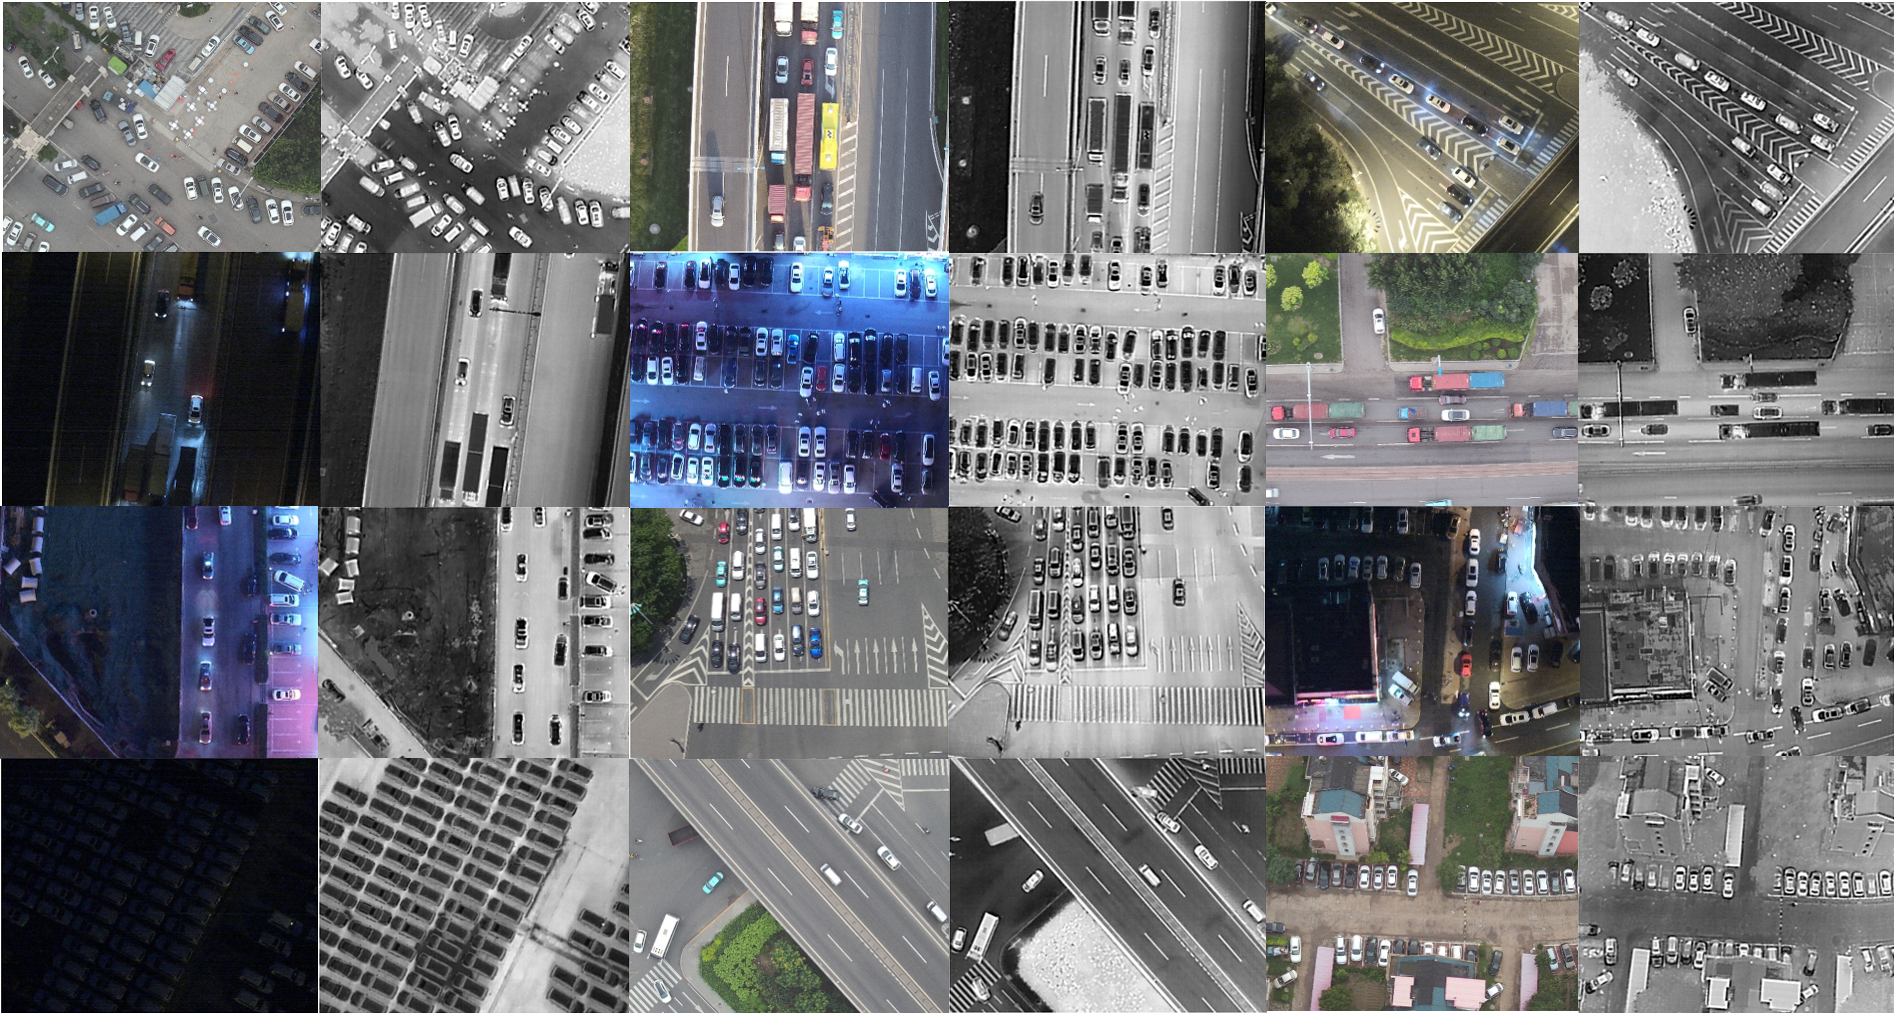
\includegraphics[width=0.85\textwidth]{dronevehicle-exem.png}
\caption{DroneVehicle数据集示例}
\label{dronevehicle-exem}
\end{figure}

\xsubsection{评价指标}{Task of Trajectory Prediction}
评价指标为理解模型的能力边界与优化方向提供了标准化的度量框架,经过多年发展,研究者们定义了一系列标准化的评价指标,本节将系统梳理目标检测领域的核心评价指标,阐述其计算原理及其在算法评估中的具体意义。

一个预测框是否正确通过计算预测框与真值框的交并比(Intersection over Union, IoU)来确定,其定义为预测框与真值框的交集面积与并集面积之比:

\begin{equation}
    \text{IoU} = \frac{\text{Area of Overlap}}{\text{Area of Union}} = \frac{B_{pred} \cap B_{gt}}{B_{pred} \cup B_{gt}}
\end{equation}

早期标准中认为预测框与真值框IoU大于0.5即为正确。然而,随着检测算法性能的提升,单一的IoU阈值已无法全面反映模型在不同定位精度下的表现。为此,后续评测标准引入了多阈值评估机制,如COCO数据集采用从0.5到0.95(步长为0.05)的10个IoU阈值,计算平均精度,以更细粒度地衡量模型在不同定位要求下的性能。

在构建评估指标之前,通常需要根据预测结果与真实标签的对应关系,统计四种预测结果:真正例(True Positive, TP)、假正例(False Positive, FP)、 真负例(True Negative, TN)和假负例(False Negative, FN)。如图\ref{confus-matrix}所示,通过这四类预测情况可以构成混淆矩阵(Confusion Matrix)来可视化模型的分类性能。

\begin{figure}[H]
\centering
\includegraphics[width=0.5\textwidth]{confus-matrix.png}
\caption{预测结果混淆矩阵}
\label{confus-matrix}
\end{figure}

基于以上四种情况,可以定义一系列核心评价指标:

\subsubsection{精确率(Precision)}
精确率表示模型预测为正的样本中实际为正类的比例,定义为:
\begin{equation}
    \text{Precision} = \frac{TP}{TP + FP}
\end{equation}

\subsubsection{虚警率(False Positive Rate, FPR)}
虚警率表示模型预测为正的样本中实际为负类的比例,定义为:
\begin{equation}
    \text{FPR} = \frac{FP}{TP + FP}
\end{equation}

\subsubsection{召回率(Recall)}
召回率表示模型正确识别出的正样本占所有实际正样本的比例,定义为:
\begin{equation}
    \text{Recall} = \frac{TP}{TP + FN}
\end{equation}

\subsubsection{平均精度(Average Precision, AP)}
平均精度是通过计算不同召回率下的精确率曲线下面积来衡量模型整体性能的指标。具体计算方法为:
\begin{equation}
    \text{AP} = \int_0^1 \text{Precision}(r) \, dr
\end{equation}
其中,$\text{Precision}(r)$表示在召回率$r$下的精确率。AP值越高,表示模型在不同召回率下的精确率表现越好,这里的AP是对单个类别计算,衡量模型对某一个类别的检测能力。

\subsubsection{平均精度均值(Mean Average Precision, mAP)}
平均精度均值是对所有类别的平均精度进行平均得到的指标,定义为:
\begin{equation}
    \text{mAP} = \frac{1}{N} \sum_{i=1}^{N} \text{AP}_i
\end{equation}
其中,$N$为类别总数,$\text{AP}_i$为第$i$类的平均精度。mAP值越高,表示模型在所有类别上的整体性能越好。

在PASCAL VOC评价体系中,AP与mAP是两个独立的指标,mAP是所有类别AP的平均值,在COCO数据集评价体系中,只保留了AP的概念,但是这里的AP的计算方式实际是PASCAL VOC中的mAP,并且更加精细化,即对所有类别和多个IoU阈值下的AP进行平均。


\xsection{单目标跟踪算法概述}{Overview of Single Object Tracking Algorithms}

单目标跟踪(Single Object Tracking, SOT)是指在视频序列中持续追踪一个指定目标的位置和状态。近年来,基于深度学习的单目标跟踪算法取得了显著进展。主流的单目标跟踪算法可以分为两大类:基于相关滤波器的方法和基于深度神经网络的方法。基于相关滤波器的方法,如KCF(Kernelized Correlation Filters)\cite{henriques2015high}和DSST(Discriminative Scale Space Tracker)\cite{danelljan2014accurate},通过在频域中进行高效的相关运算,实现了实时的目标跟踪。基于深度神经网络的方法,如Siamese网络系列\cite{bertinetto2016fully, li2018high, valmadre2017end},通过学习目标的深度特征表示,提高了跟踪的鲁棒性和准确性。此外,近年来引入注意力机制和Transformer架构的跟踪算法,如SiamRPN++\cite{li2019siamrpn++}和TransT\cite{chen2021transformer},进一步提升了跟踪性能。多光谱单目标跟踪算法通过融合可见光和红外图像信息,提高了在复杂环境下的跟踪鲁棒性。常见的多光谱融合方法包括特征级融合、决策级融合和输入级融合等。


\xsection{本章小结}{Chapter Summary}

本章介绍了智能光电系统中的核心功能——目标识别和单目标跟踪的相关算法基础知识。目标识别算法主要分为一阶段检测器和二阶段检测器两大类,近年来Transformer架构也被引入该领域。单目标跟踪算法则包括基于相关滤波器的方法和基于深度神经网络的方法,近年来注意力机制和Transformer架构的引入进一步提升了跟踪性能。此外,多光谱融合技术在目标识别和单目标跟踪中发挥了重要作用,提高了算法在复杂环境下的鲁棒性。下一章将详细介绍多光谱融合智能光电处理算法的设计与实现。